\section{Dust Empirical Modeling} \label{sec:dem}
In this section we present the dust empirical model (DEM), a flexible model for
applying attenuation curves to galaxy populations that allows us to incorporate
intrinsic variations in dust attenuation as well as correlation to physical
galaxy properties. Later, we demonstrate that we can accurately reproduce
observations with the DEM and use it to test galaxy formation models and shed
light on dust in galaxies. 

We define the dust attenuation curve $A(\lambda)$ as 
\begin{equation} 
    F_o (\lambda) = F_i (\lambda) 10^{-0.4 A(\lambda)}
\end{equation}
where $F_o$ is the observed flux and $F_i$ is the intrinsic flux. We normalize
the attenuation at the $V$ band, 
\begin{equation} 
    A(\lambda) = A_V \frac{k(\lambda)}{k_V}
\end{equation}
so that $A_V$ determines the amplitude of the attenuation, while $k(\lambda)$
determines the wavelength dependence. 

To determine $A(\lambda)$ for each galaxy, we first assign $A_V$ using the slab
model from~\cite{somerville1999, somerville2012}. In the slab model, $A_V$ is
calculated from the inclination of the galaxy, $i$, and its optical depth, $\tau_V$: 
\begin{equation} \label{eq:slab}
    A_V = -2.5 \log \left[ \frac{1 - e^{-\tau_V\,\sec i}}{\tau_V\,\sec i} \right].
\end{equation}
For all of our galaxies, we uniformly sample $i$. Then, we include the
correlation between $A_V$ and galaxy properties ($M_*$ and $\sfr$), found
in both observations and simulations~\citep[\eg][]{narayanan2018, salim2020},
in $\tau_V$. We use $\tau_V$ with a simple and flexible linear $M_*$ and $\sfr$ 
dependence:
\begin{equation} \label{eq:tauv}
    \tau_V(M_*, \sfr) = \mtaum \log \left(\frac{M_*}{10^{10} M_\odot}\right) + \mtaus \log\,\sfr + c_\tau.
\end{equation}
$\mtaum$ quantifies the $M_*$ dependence, $\mtaus$ quantifies the $\sfr$
dependence, and $c_\tau$ quantifies the overall amplitude. Since $\tau_V$ is
optical depth, we impose a $\tau_V \ge 0$ limit. We note that the slab model 
is a naive approximation. In reality, $A_V$ for a galaxy will depend on complexities 
of its star-to-dust geometry, variations in the extinction curves, and other
properties beyond just inclination and $\tau_V$. The purpose of the DEM,
however, is not to accurately model dust attenuation for individual galaxies,
but rather to accurately model the distribution of dust attenuation of galaxy
populations. In this sense, the slab model qualitatively reproduces the
correlation between $A_V$ and $i$ found in the literature: edge-on galaxies
have higher $A_V$ than face-on galaxies~\citep[\eg][]{salim2020}. More
importantly, the distribution of $A_V$, $p(A_V)$, produced using the slab model with
uniformly sampled inclinations closely matches the $p(A_V)$ of our SDSS sample
(Figure~\ref{fig:av_dist}). Also, we demonstrate that replacing the slab model
with a more flexible prescription for sampling $A_V$ does not significant
impact our analysis (Appendix~\ref{sec:nonslab}). We therefore conclude that
the slab model is a sufficiently flexible empirical prescription for sampling
$A_V$. 

Next, for the wavelength dependence of the attenuation curve, we use the
parameterization of $k(\lambda)$ from \cite{noll2009}: 
\begin{equation} \label{eq:noll}
    k(\lambda) = \left(k_{\rm Cal}(\lambda) + D(\lambda)\right) \left(
    \frac{\lambda}{\lambda_V} \right)^\delta.
\end{equation}
Here $k_{\rm Cal}(\lambda)$ is the \cite{calzetti2001} curve: 
\[
    k_{\rm Cal}(\lambda) = 
    \begin{cases} 
        2.659 (-1.857 + 1.040/\lambda) + R_V, & 6300 \AA \le \lambda \le
        22000 \AA \\ 
        2.659 (-2.156 + 1.509/\lambda - 0.198/\lambda^2 + 0.011/\lambda^3) +
        R_V & 1200 \AA \le \lambda \le 6300 \AA
    \end{cases}
\]
where $\lambda_V = 5500 \AA$ is the $V$ band wavelength. $\delta$ is the slope
offset of the attenuation curve from $k_{\rm Cal}$. Given the evidence that
$\delta$ correlate with galaxy properties~\citep[\eg][]{leja2017, salim2018},
we parameterize $\delta$ with a similar $M_*$ and $\sfr$ dependence as
$\tau_V$:  
\begin{align}
    \delta(M_*, \sfr) &= \mdeltam \log \left(\frac{M_*}{10^{10}
    M_\odot}\right) + \mdeltas \log\,\sfr + c_\delta 
\end{align}
$D(\lambda)$ in Eq.~\ref{eq:noll} is the UV dust bump, which we parameter using
the standard Lorentzian-like Drude profile:
\begin{equation}
    D(\lambda) = \frac{E_b(\lambda \Delta \lambda)^2}{(\lambda^2 -
    \lambda_0^2)^2 + (\lambda \Delta \lambda)^2}
\end{equation}
where $\lambda_0$, $\Delta \lambda$, and $E_b$ are the central wavelength,
FWHM, and strength of the bump, respectively. In our DEM, we assume fixed 
$\lambda_0 = 2175 \AA$ and $\Delta \lambda = 350\AA$. 

% Although a number of works have found correlation between the attenuation
% curve slope and inclination~\citep{wild2011, chevallard2013, battisti2017b},
% \cite{salim2020}, most recently, found that the driver of this trend is the
% relationship between $A_V$ and slope. We therefore do not include an
% inclination dependence in $\delta$. 

\cite{kriek2013} and \cite{tress2018} found evidence that $E_b$ correlates with
the slope of the attenuation curve for star-forming galaxies $z\sim2$. This was
dependence was confirmed with simulations in \cite{naranyanan2018}. $E_b$: 
\begin{align} \label{eq:bump_amp}
    E_b &= m_E~\delta + c_E
\end{align}
\todo{we fixed this and find our results do not change significantly.} 

We also split the attenuation on the star light and nebular emission 
\begin{equation} 
    F_o (\lambda) = F^{\rm star}_i (\lambda) 10^{-0.4 A(\lambda)} + F^{\rm
    neb}_i (\lambda) 10^{-0.4 A_{\rm neb}(\lambda)}
\end{equation}
where we parameterize
\begin{equation}
    A_{\rm neb}(\lambda) = f_{\rm neb}  A(\lambda) 
\end{equation} 

\todo{mention of how we treat SFR = 0 galaxies} 

\begin{figure}
\begin{center}
    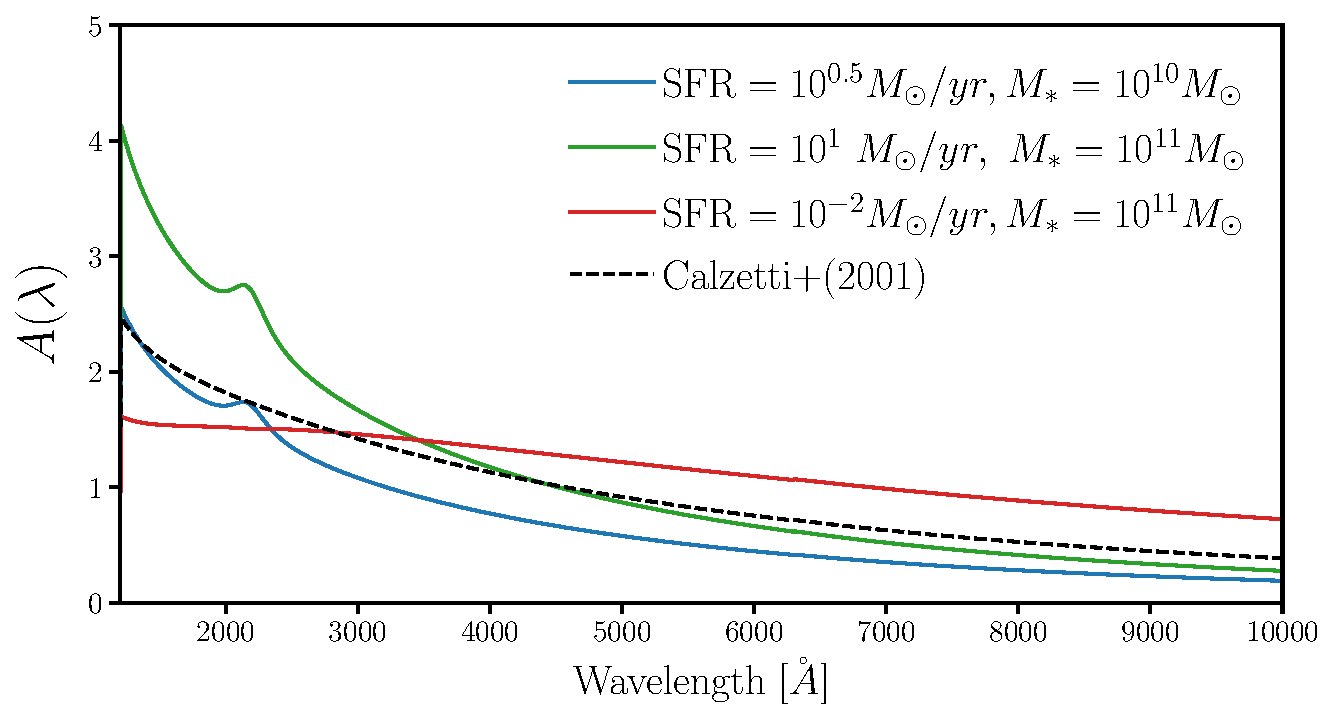
\includegraphics[width=0.6\textwidth]{figs/dems.pdf}
    \caption{Comparison of the attenuation curve for our fiducial dust empirical
    model (DEM; black) to common attenuation curves in the
    literature (\citealt{calzetti2001}, orange; \citealt{salim2018}, blue). We compare the curves for typical 
    star-forming galaxies with ${\rm SFR}=10^{0.5}M_\odot/yr$ in the left panel
    and for quiescent galaxies with ${\rm SFR}=10^{-2}M_\odot/yr$ in the right.
    For our fiducial DEM, we use parameter values at {\color{red} the center of the priors
    listed in Table~\ref{tab:free_param}} and include attenuation curves for $M_* = 10^{9.5}$
    (dashed) and $10^{11} M_\odot$ (solid). {\em Our fiducial DEM is flexibly
    parameterized to incorporate both $M_*$ and SFR dependence in the
    attenuation curve} (Section~\ref{sec:dem}).
    } 
\label{fig:dem}
\end{center}
\end{figure}


%%%%%%%%%%%%%%%%%%%%%%%%%%%%%%%%%%%%%%%%%%
% table of free parameters
%%%%%%%%%%%%%%%%%%%%%%%%%%%%%%%%%%%%%%%%%%
\begin{table}
    \caption{Parameters of the Dust Empirical Models}
    \begin{center}
        \begin{tabular}{ccc} \toprule
            Parameter & Definition & prior\\[3pt] \hline\hline
            %\multicolumn{3}{c}{DEM with slab model}\\ \hline
            $m_{\tau,M_*}$ & Slope of the $\log M_*$ dependence of optical depth,
            $\tau_V$ & flat $[-5., 5.]$\\
            $m_{\tau,{\rm SFR}}$ & Slope of the $\log {\rm SFR}$ dependence of optical depth, $\tau_V$ & flat $[-5., 5.]$\\
            $c_{\tau}$ & amplitude of the optical depth, $\tau_V$ & flat $[0., 6.]$\\
            %\hline
            %\multicolumn{3}{c}{DEM with $\mathcal{N}_T$ model}\\ \hline
            %$m_{\mu,1}$ & Slope of the $\log M_*$ dependence of optical depth,
            %$\tau_V$ & flat $[-5., 5.]$\\
            %$m_{\mu,2}$ & Slope of the $\log {\rm SFR}$ dependence of optical
            %depth, $\tau_V$ & flat $[-5., 5.]$\\
            %$c_{\mu}$ & amplitude of the optical depth, $\tau_V$ & flat $[0., 6.]$\\ 
            %$m_{\sigma,1}$ & Slope of the $\log M_*$ dependence of optical depth, $\tau_V$ & flat $[-5., 5.]$\\
            %$m_{\sigma,2}$ & Slope of the $\log {\rm SFR}$ dependence of optical depth, $\tau_V$ & flat $[-5., 5.]$\\
            %$c_{\sigma}$ & amplitude of the optical depth, $\tau_V$ & flat $[0.1, 3.]$\\ 
            %\hline
            $m_{\delta,1}$ & Slope of the $\log M_*$ dependence of the
            attenuation curve slope offset, $\delta$ & flat $[-4., 4.]$\\
            $m_{\delta,2}$ & Slope of the $\log {\rm SFR}$ dependence of the
            attenuation curve slope offset, $\delta$ & flat $[-4., 4.]$\\
            $c_{\delta}$ & amplitude of the attenuation curve slope offset, $\delta$ & flat $[-4., 4.]$\\
            %$m_{E}$ & slope of the $\delta$ dependence of UV dust bump strength, $E_b$ & flat $[-4., 0.]$\\
            %$c_{E}$ & amplitude of UV dust bump strength, $\delta$ & flat $[0., 4.]$\\
            $f_{\rm neb}$ & fraction of nebular attenuation curve & flat $[1., 4.]$\\
            \hline
        \end{tabular} \label{tab:free_param}
    \end{center}
\end{table}
%%%%%%%%%%%%%%%%%%%%%%%%%%%%%%%%%%%%%%%%%%

\section{Likelihood-Free Inference} \label{sec:abc}
Approximate Bayesian Computation with Population Monte Carlo \cite{hahn2017a},

We also restrict the
sample to central galaxies where brighter than $M_r < -20$, where our SDSS 
central galaxy sample is complete. 



To compare the outputs of our DEMs to observations, we first measure the color-magnitude
observables ($G-R$, $FUV-NUV$, and $M_r$) as described in Section~\ref{sec:fm}
consistent with SDSS measurements. Afterwards, we compare the forward modeled
observables to SDSS using a L2 norm distance metric: 
\begin{equation}
    \bar{\rho}(\theta) = \sum\limits_{i=1}^{n} \left[X^{\rm SDSS}_i - X^{\rm model}_i(\theta) \right]^2.
\end{equation}
$X^{\rm SDSS}$ and $X^{\rm model}(\theta)$ are $n$-dimensional data vectors of
the SDSS and model observables. In our case, we use a 3-dimensional histogram
along $G-R$, $FUV-NUV$, 

\cite{ishida2015} 

Paragraph on the priors we choose. 
\begin{itemize}
    \item flat priors on everything. We might want to note that this doesn't
        give flat priors on $\tau_V$ or $\mu_{A_V}$ and $\sigma_{A_V}$ for NT
        but we're ultimately interested in the dependence. 
    \item priors were chosen to be uniformative and encompass constraints in
        the literature:
    \item $m_E$ and $c_E$ were chosen to be include \cite{kriek2013, narayanan2018, tress2018} 
\end{itemize}
